\documentclass[10pt]{article}
\usepackage[utf8]{inputenc}
\usepackage{empheq}
\usepackage[inline, shortlabels]{enumitem}
\usepackage{gensymb}
\usepackage{multicol}
\setlength{\parskip}{0.5cm plus4mm minus3mm}
\setlength{\parindent}{0pt}
\usepackage{amsmath}
\usepackage{upgreek}
\usepackage[nobreak=true]{mdframed}
\usepackage[margin=0.6in]{geometry}
 \geometry{
 left=12mm,
 bottom=20mm
 }
\usepackage{amssymb}
\usepackage{cs170}
\usepackage{titlesec}
\usepackage{chngcntr}
\usepackage{graphicx}
\usepackage{changepage}
\usepackage{chngcntr}
\usepackage{scrextend}
\usepackage{minted}
\usemintedstyle{colorful}

\begin{document}
\date{}
\title{\vspace{-5ex} \dunhd{CS70: Discrete Math and Probability Theory Notes} \vspace{-5ex}}
\maketitle
\begin{multicols}{2}
\begin{enumerate}
    \item \textbf{Sets} 
    \begin{enumerate}
        \item In mathematics, a \textbf{set} is a well-defined collection of distinct objects. The \textbf{cardinality}, or size, of a set $A$ is denoted by $|A|$. If $x$ is an element of $A$, we denote membership by $x \in A$.
         \item If every element of a set $A$ is also in set $B$, then we say that $A$ is a \textbf{subset} of $B$, written $A \subseteq B$. 
         \item Two sets $A$ and $B$ are said to be \textbf{equal} if $A \subseteq B$ and $B \subseteq A$.
         \item A \textbf{proper subset} is a set $A$ that is strictly contained in $B$, written as $A \subset B$, meaning that $A$ excludes at least one element of $B$. 
         \item The \textbf{intersection} of a set $A$ with a set $B$, written as $A \cap B$, is a set containing all elements which are in both $A$ and $B$. 
         \item The \textbf{union} of a set $A$ with a set $B$, written as $A \cup B$, is a set of all elements which are in either $A$ or $B$ or both. 
         \item The \textbf{relative complement} of $A$ in $B$, written as $B - A$ or $B \setminus A$, is the set of elements in $B$, but not in $A$.
         \item The \textbf{Cartesian product} of $A$ and $B$, written $A \times B$, is the set of all ordered pairs $\{(a,b) \mid a \in A, b \in B \}$.
    \end{enumerate}

    
    \item \textbf{Important Sets} 
    \begin{itemize}
        \item $\mathbb{N}$ denotes the set of all natural numbers: $\left\{0,1,2,3,\hdots \right\}$.
        \item $\mathbb{Z}$ denotes the set of all integer numbers: $\left\{\hdots,-2,-1,0,1,2,\hdots\right\}$. 
        \item $\mathbb{Q}$ denotes the set of all rational numbers: $\left\{ \frac{a}{b} \mid a,b \in \mathbb{Z}, b \neq 0 \right\}$.
        \item $\mathbb{R}$ denotes the set of all real numbers.
        \item $\mathbb{C}$ denotes the set of all complex numbers.
    \end{itemize}
    
    \item \textbf{Propositional Logic}
    \begin{enumerate}
        \item A \textbf{proposition} is a declaration that is either true or false. Two propositions $P$ and $Q$ are logically equivalent, denoted $P \equiv Q$, if they share the same truth values.
        \item Connectives: 
        \begin{align*}
            \text{And}: P \land Q \hspace{8mm} \text{Or}: P \lor Q \hspace{8mm} \text{Not}: \neg P 
        \end{align*}
         Quantifiers: 
         \begin{align*}
             \text{There exists}: \exists \hspace{8mm} \text{For all}: \forall
         \end{align*}
        \item \textbf{Implication:} “If $P$, then $Q$", denoted $P \implies Q$. This is logically equivalent to $\neg P \lor Q$. (Note that implication is only false when $P$ is true and $Q$ is false)
         

        \item The \textbf{contrapositive} of $P \implies Q$ is $\neg Q \implies \neg P$, which is logically equivalent.
        \item The \textbf{converse} of $P \implies Q$ is $Q \implies P$, which is \textit{not} logically equivalent. 
        \item \textbf{If and only if} (iff), denoted $P \iff Q$, is equivalent to implication in both directions: $(P \implies Q) \land (Q \implies P)$.
        \item \textbf{Distribution Laws:} \\ $P \land (Q \lor R) \iff (P \land Q) \lor (P \land R)$ \\
         $P \lor (Q \land R) \iff (P \lor Q) \land (P \lor R)$
        
        \item \textbf{DeMorgan's Laws} \\ $\neg (P \lor Q) \iff \neg P \land \neg Q$ \\
         $\neg (P \land Q) \iff \neg P \lor \neg Q$ \\
         $\neg (\forall x P(x)) \iff \exists x (\neg P(x))$ \\
         $\neg (\exists x P(x)) \iff \forall x (\neg P(x))$ 
        \item Equivalencies: \\
        $\forall x (P(x) \land Q(x)) \iff (\forall x,P(x)) \land (\forall x,Q(x))$ \\
        $\exists x (P(x) \lor Q(x)) \iff (\exists x,P(x)) \lor (\exists x,Q(x))$
    \end{enumerate}
    
    \item \textbf{Formal Definitions and Important Lemmas}
    \begin{enumerate}
        \item Given integers $a$ and $b$, we say that $a$ divides $b$, denoted $a|b$, (or $b$ is divisible by $a$) iff there exists an integer $q$ such that $b = aq$.
        \item A prime number is divisible only by 1 and itself.
        \item An even number is an integer $n$ of the form $n=2k, k \in \mathbb{Z}$. An odd number is an integer $n$ of the form $n=2k+1, k \in \mathbb{Z}$.
        \item If $a^2$ is even, then $a$ is even.
        \item Every natural number greater than one is either prime or has a prime divisor.
        \item The well-ordering principle states that every non-empty set of positive integers contains a least element. 
    \end{enumerate}
    
    \item \textbf{Proof techniques}
    \begin{enumerate}
        \item \textbf{Direct proof:} Goal: Prove $P \implies Q$. Assume $P$ $\hdots$ therefore $Q$. Often involves appealing to definitions and using algebraic manipulations.
        \item \textbf{Proof by contraposition:} Goal: Prove $P \implies Q$. Assume $\neg Q$ $\hdots$ therefore $\neg P$.
        \item \textbf{Proof by contradiction:} Goal: Prove $P$. Assume $\neg P$. Show that $\neg P \implies R \land \neg R$, a contradiction. Therefore, $P$.
        \item \textbf{Proof by cases:} In proving a claim, we don’t know which of a set of possible cases is true, but we know that at least one of the cases is true. What we can do then is to prove the result in both cases; then, clearly the general statement must hold.
        \item \textbf{Proof by induction:} Goal: Prove $P$. Choose an appropriate quantity $n$ to induct on. In the \textit{base case}, show that $P(1)$ is true. In the inductive hypotheses, assume $P(k)$ is true for some $k \geq 1$. In the inductive step, show that the claim holds for $P(k+1)$. Conclude that $P$ holds for all $n$.
        \item \textbf{Strong induction:} Same as induction, but with stronger inductive hypotheses: Assume $P(j)$ is true for all $1 \leq j \leq k$ for some $k$. Then show that $P(k+1)$ is true.
    \end{enumerate}
    
    \item \textbf{Stable Marriage algorithm:} Each man and woman has an ordered preference list of their $n$ potential partners. The algorithm is as follows: 
    \begin{enumerate}
        \item Each man proposes to the most preferred woman on his list who has not yet rejected him.
        \item Each woman collects all the proposals she received; to the man she likes best, she responds “maybe” (puts him on a string), and to the others, she says “never”.
        \item Each rejected man crosses off the woman who rejected him from his list.
    \end{enumerate}
    Repeat until each women has a man on a string. \\
    Properties of the algorithm:
    \begin{enumerate}
        \item It outputs a stable pairing, meaning there are no rogue couples (a man and a woman who prefer each other to their current partners). It is not necessarily the only stable pairing.
        \item The algorithm must terminate in at most $n^2$ days (precisely, $n^2-2n+2$).
        \item (Improvement lemma) If man $M$ proposes to woman $W$ on the $k^{th}$ day, then on every subsequent day $W$ has someone on a string whom she likes at least as much as $M$.
        \item (Male optimal and Female pessimal) It outputs a pairing such that each man is paired with his optimal woman (the most preferred woman a man can stably end up with). 
    \end{enumerate}
    
    \item \textbf{Graph Theory} 
    \begin{enumerate}
        \item An \textit{undirected} graph $G$ is defined by a set of vertices $V$ and a set of edges $E$ consisting of pairs of vertices. A \textit{directed} graph models one-way relationships, so we have $E \subseteq V \times V$.
        \item The edge $e = \{u, v \}$ is \textit{incident} on vertices $u$ and $v$, and we say $u$ and $v$ are \textit{adjacent}. If $G$ is undirected, then the \textit{degree} of vertex $u \in V$ is the number of edges incident to $u$. If $G$ is directed, $u$ has an associated \textit{in-degree} and \textit{out-degree}.
        \item Let $G$ be an undirected graph. A \textbf{path} in $G$ is a sequence of edges with no repeated vertices or edges (simple). A \textbf{cycle} is a path which starts and ends on the same vertex. A \textbf{walk} is a sequence of edges which can have repeated vertices. A \textbf{tour} is a walk which starts and ends at the same vertex. \textbf{Connected components} are sets $V_1,\hdots,V_k$ of vertices, such that all vertices in a set $V_i$ are connected.
        \item A Eulerian walk is a walk in $G$ that uses each edge exactly once (Eulerian tour if ends at same vertex). \textit{Theorem:} An undirected graph $G$ has a Eulerian tour iff $G$ is even degree and connected (except for isolated vertices). 
        \item A recursive algorithm for Eulerian Tour is as follows:
        \begin{minted}[linenos=false, escapeinside=??, mathescape=true]{octave}
function Euler(?$G,s$?): 
    T = findTour(?$G,s$?) 
    return splice(T, Euler(?$G_1, s_1$?), ?$\hdots$?, 
                     Euler(?$G_k, s_k$?))
        \end{minted}
        where \texttt{findTour}($G,s$) finds any tour in $G$ from $s$; $G_1, \hdots,G_k$ are the connected components when the edges in $T$ are removed from $G$; $s_i$ is the first vertex in $T$ that intersects $G_i$; and \texttt{splice} returns a combined tour obtained by traversing the edges of $T$ such that whenever it reaches a vertex $s_i$ that intersects another tour $T_i$, it takes a detour to traverse $T_i$ from $s_i$ back to $s_i$ again.
        \item A graph is a \textbf{tree} if it is connected and acyclic. Equivalent definitinions include: There are $v-1$ edges; the removal of any edge disconnects the graph; the addition of any edge creates a cycle. Unique path between any pair of vertices. Note that a tree must contain a degree 1 node (called a leaf).
        \item A graph is \textbf{planar} if it can be drawn on the plane without crossings. \textbf{Faces} $f$ are the regions into which the graph subdivides the plane. 
        \item Euler's Formula: For every connected planar graph, $v+f=e+2$. Important consequence: $e \leq 3v-6$ (Planar graphs are sparse).
        \item A graph is non-planar if and only if it contains $K_5$ or $K_{3,3}:$
        \begin{align*}
            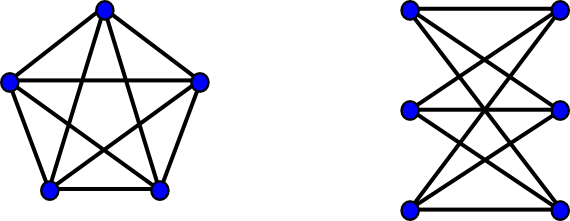
\includegraphics[width=4cm]{kk.png}
        \end{align*}
        (Contains means that one can identify nodes in the graph which are connected as $K_5$ or $k_{3,3}$ through paths such that each two of these paths share a vertex.)
        \item A \textbf{bipartite graph} is a graph whose vertices can be divided into two disjoint sets (no shared elements) $U$ and $V$ such that \textit{every} edge connects a vertex in $U$ to a vertex in $V$.
        \item A \textbf{complete graph} is a graph in which all nodes are connected to all other nodes. Let $K_n$ denote the unique complete graph for $n$ vertices. $K_n$ has $n(n-1)/2$ edges.
        \item Useful facts: 
        \begin{enumerate}
            \item By definition of a cycle, removing any edge in the cycle does not disconnect the graph $G$.
            \item If $G$ is connected, then the addition of any vertex incident on more than one edge will create a cycle.
            \item The sum of the degrees of all vertices in a graph is $2|E|$ (twice the number of edges).
            \item In proofs relating to the maximum degree of a graph, do induction on the number of edges or vertices (with fixed maximum degree).
        \end{enumerate}
        \item \textbf{Hypercubes:} 
        
        The vertex set of the n-dimensional hypercube $G = (V,E)$ is given by $V = \{0,1\}^n$, where $\{0,1\}^n$ denotes the set of all $n$-bit strings. There are $2^n$ vertices and $n2^{n-1}$ edges. Two vertices $x$ and $y$ are connected by edge $\{x,y\}$ if and only if $x$ and $y$ differ in exactly one bit position.
        \begin{align*}
           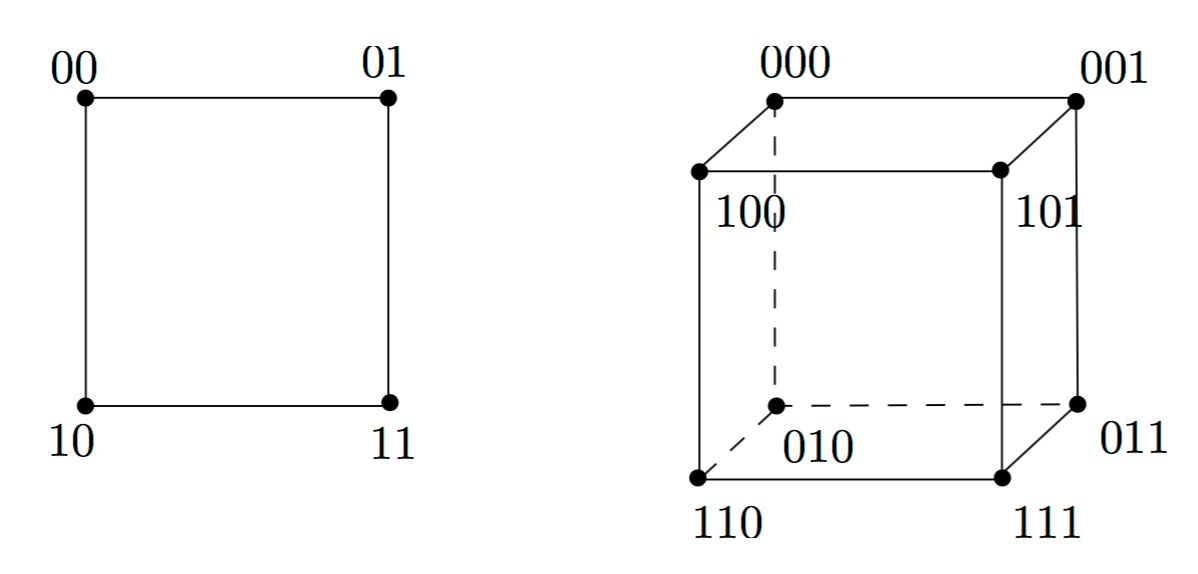
\includegraphics[scale=0.25]{cube2.png}
        \end{align*}
        \textbf{Recursive definition} of hypercube: Define the 0-subcube and 1-subcube as the $(n-1)$-dimensional hypercube with vertices labeled by 0$x$ for $x \in \{0,1\}^{n-1}$ and 1$x$ for $x \in \{0,1\}^{n-1}$, respectively. Then, the $n$-dimensional hypercube is obtained by placing an edge between each pair of vertices 0$x$ in the 0-subcube and 1$x$ in the 1-subcube.

    \end{enumerate}
    
    \item \textbf{Modular Arithmetic} 
    \begin{enumerate}
        \item $x$ (mod $n$) = $x - (\left \lfloor{\frac{x}{n}}\right \rfloor n)$
        \item We can perform any sequence of arithmetic operations $\pmod{n}$ and the result remains unchanged whether we reduce by $\pmod{n}$ only once at the end of all operations, or we reduce each intermediate result by $\pmod{n}$.
        \item For two integers $a$ and $b$, we define $a$ to be congruent to $b$ modulo $n$ ($a \equiv_n b$) iff: \\
            $\iff a \pmod{n} = b \pmod{n}$ \\ $\iff n | (a-b)$ \\ $\iff a = b+kn$
        \item For all $n \geq 1$ and $a,b,c,d \in \mathbb{Z}$, if $a \equiv_n b$ and $c \equiv_n d$, then
        \begin{enumerate}
            \item $a + c \equiv_n b + d$
            \item $a - c \equiv_n b - d$
            \item $ac \equiv_n bd$
        \end{enumerate}
        \item The \textbf{multiplicative inverse} of $x \pmod{n}$ is $y$ such that $xy\pmod{n} = 1$. \textit{Theorem:} $x$ has a multiplicative inverse modulo $n$ if and only if $\gcd(x,n)=1$. Moreover, this inverse is unique.
        \item We note that if $x \geq y$, then $\gcd(x,y)=\gcd(y, x$ $\pmod{y}$). This allows to write the following extended $\gcd$ algorithm for $x \geq y \geq 0$ and $x > 0$:
        \begin{minted}[linenos=false, escapeinside=??, mathescape=true]{octave}
function extendedGCD(?$x,y$?)
if ?$y = 0$?:
    return (?$x,1,0$?)
gcd, ?$a$?, ?$b$? = extendedGCD(?$y,x \pmod{y}$?)
return (gcd, ?$b$?, ?$a - \lfloor \frac{x}{y} \rfloor b$?)
        \end{minted}
        It returns ($\gcd, a, b$) such that $\gcd$ is $\gcd(x,y)$ and $a$,$b$ satisfy $\gcd = ax + by$. Thus $b$ is the multiplicative inverse of $x$ (mod $n$).
        
        
        This algorithm uses $2n$ divisions, where $n$ is the number of bits (an integer $x$ requires $\lfloor{log_2(x)} \rfloor+1)$ bits).
    \end{enumerate}
    
    \item \textbf{Bijections}
    \begin{enumerate}
        \item A \textbf{function} $f: A \mapsto B$ maps values from a domain $A$ to a range $B$. A function $f$ is \textbf{bijective} iff it is \textbf{surjective} (onto): $\forall b \in B, \exists a \in A$ such that $f(a)=b$; and \textbf{injective} (one-to-one): $\forall a,a' \in A$, if $f(a)=f(a')$, then $a=a'$. 
        \item \textit{Lemma:} A function $f: A \mapsto A$ is a bijection iff there is an inverse function $g: A \mapsto A$ such that $f(g(x))=x$ and $g(f(y))=y$ $\forall x,y \in A$.
        \item \textbf{Fermat's Little Theorum:} For any prime $p$ and any $a \in \mathbb{Z}$, $a^p \equiv a \pmod{p}$. If $a$ is not divisble by $p$, such as if $a \in \{1,2,\hdots,p-1\}$, then we have $a^{p-1} \equiv 1 \pmod{p}$.
    \end{enumerate}
    
    \item \textbf{RSA}
    \begin{enumerate}
        \item RSA is a form of public key encryption which uses an easy-to-compute but difficult to invert (without the key) bijection.
        \item Encryption $E: \{0,\hdots,N-1\} \mapsto \{0,\hdots,N-1\}$ is given by $$E(x)=x^e \pmod{N}$$ where $N=pq$ for two large primes $p$ and $q$ and $e$ is relatively prime to $(p-1)(q-1)$.
        \item Decryption is given by $$D(x)=x^d \pmod{N}$$ where $d$ is the multiplicative inverse of $e \pmod{(p-1)(q-1)}$.
        \item To show that RSA works, we show that $D(E(x))=x$, that is, $x^{ed} \equiv x \pmod{N}$, or $x^{ed} - x \equiv 0 \pmod{N}$ for $x \in\{0,1, \ldots, N-1\}$. Since $ed \equiv 1 \pmod{(p-1)(q-1)}$, or written another way, $ed = 1 + k(p-1)(q-1)$ for some integer $k$, we get $x^{ed} - x = x^{1 + k(p-1)(q-1)} - x = x(x^{k(p-1)(q-1)})$. If $x$ is a multiple of $p$, then clearly the claim follows. If not, use Fermat's Little Theorem to see the claim still follows. 
        \item When we have to compute $x^y \pmod{N}$ for some large $y$, we use a simple technique known as repeated squaring to keep the number of multiplications $O(\log y)$ instead of $O(y)$.
        \item RSA is secure because given $N$, $e$, and $E(x)$, there is no efficient algorithm for finding $x$. (Amounts to factoring $N$ into $p$ and $q$). $p$ and $q$ are often over 100 digits.
    \end{enumerate}
    \item \textbf{Polynomials} 
    \begin{enumerate}
    \item A single-variable \textbf{polynomial} of degree $d$ is a function of the form $$p(x)=a_dx^d+a_{d-1}x^{d-1}+\hdots+a_0$$ \item $a$ is a root of $p(x)$ iff $p(a)=0$.
    \item \textbf{Property 1:} A degree $d$ polynomial has at most $d$ roots. \\
    \textit{Proof:} This follows from the following facts:
    \begin{itemize}
        \item If $a$ is a root of $p(x)$ with degree $d$, then $p(x) = (x - a)q(x)$ for a polynomial $q(x)$ with degree $d - 1$. (We use the result from polynomial division and show $r(x)=0$).
        \item A polynomial $p(x)$ of degree $d$ with distinct roots $a_1,\hdots,a_d$ can be written as $p(x)=c(x-a_1) \ldots (x-a_d)$.
    \end{itemize}
    \item \textbf{Property 2:} Given $d+1$ pairs $(x_1,y_1),\hdots,$ $(x_{d+1}, y_{d+1})$ of points, all $x_i$ distinct, there is a unique polynomial of (at most) degree $d$ that passes through all points. \\
    \textit{Proof:} Existence of a polynomial is proved by lagrange interpolation. Proof of uniqueness: suppose there is another such polynomial, $q(x)$. Consider a polynomial $r(x)=p(x)-q(x)$. $r(x)$ must a non-zero polynomial of degree $d$ with at most $d$ roots. But $r(x_i)=p(x_i)-q(x_i)=0$ on $d+1$ distinct points. Contradiction.
    \item \textbf{Lagrange interpolation} is a method of reconstructing the unique polynomial of degree $d$ given $d+1$ points $(x_1,y_1), \hdots,(x_{d+1}, y_{d+1})$. The lagrange polynomial is given by 
    $$p(x)=\sum_{i=1}^{d+1} y_i \Delta_i(x)$$ where
    $$\Delta_i(x)=\frac{\prod_{j \neq i} (x-x_j)}{\prod_{j \neq i} (x_i-x_j)}$$ 
    This works because when it is evaluated at $x_i$, $d$ of the $d+1$ terms in the sum go to 0 and the $i^{th}$ term becomes $y_i$ times 1, as desired. \\[8 pt]
    An alternative method is to solve a system of $d+1$ linear equations where the $i^{th}$ equation is $a_dx_{i}^{d}+a_{d-1}x_i^{d-1}+\hdots+a_0=y_i$.
    \item In \textbf{polynomial division}, if we have a polynomial of degree $d$, we can divide it by a polynomial $q(x)$ of degree $\leq d$. The result will be $$p(x)=q(x)q'(x)+r(x)$$ with $q'(x)$ the quotient and $r(x)$ the remainder with degree $< d$.
    
    \item \textbf{Finite fields} \\
    Properties 1 and 2 do not hold if the coefficients and variable $x$ are restricted to integers. But for numbers modulo a prime, we can add, subtract, multiply, and divide (by any nonzero number modulo $m$) since all the numbers have a multiplicative inverse mod $m$. When we work with numbers modulo a prime $m$, we say that we are working over a finite field, denoted by $F_m$ or $GF(m)$.
    
    \item \textbf{Counting} \\
    For polynomials of degree $\leq d$ over $F_m$: given $d+1$ points, there is exactly 1 polynomial that passes through all points. Given $d$ points, there are $m$; given $d-1$ points, there are $m^{2}$, and so on, until given 0 points, there are $m^{d+1}$.
    
    \item \textbf{Secret Sharing} \\
    We have $n$ people and a secret natural number $s$. We want to devise a scheme whereby any $k$ people can figure out $s$, but no group of $k-1$ or fewer has any information about $s$. Let $q$ be a prime larger than $n$ and $s$. We will now work over $F_q$. Pick a polynomial $P(x)$ of degree $k-1$ such that $P(0)=s$. Give $P(1)$ to the first person, $P(2)$ to the second, and so on, until you give $P(n)$ to the $n^{th}$ person. For any $k-1$ people, $s$ could be $0 \leq s \leq q-1$, but they already knew that, so they have no information about $s$. 
    \end{enumerate}
    
    \item \textbf{Error-correcting codes}
    \begin{enumerate}
        \item When transmitting information on an unreliable channel (such as the Internet), sometimes packets are lost (\textbf{erasure errors}) and sometimes packets are corrupted (\textbf{general errors}). Error-correcting codes are a method of encoding messages to prevent both of these errors.
        \item \textbf{Erasure errors:} We will work in $GF(q)$ where $q$ is a large prime. Assume the information consists of $n$ packets, denoted $m_1,\hdots,m_n$. Let $P(x)$ be the unique polynomial of degree $n-1$ such that $P(i)=m_i$ for all $1 \leq i \leq n$. We can generate $k$ additional packets by evaluating $P(x)$ at $n+1,\hdots,n+k$ (for $n+k \leq q$). The encoded message then consists of $n+k$ packets. We can reconstruct $P(x)$ from any $n$ transmitted packets, then evaluate $P(x)$ at $x=1,\hdots,n$ to obtain the original message. This scheme can protect against at most $k$ erasure errors.
        \item \textbf{General errors:} As before, we work in $GF(q)$. To guard against $k$ general errors, the encoded message must now contain $2k$ additional packets. We must now reconstruct $P(x)$ from $n+2k$ received messages, $r_1,\hdots,r_{n+2k}$. We know $P(i)$ must equal $r_i$ on at least $n+k$ points, but we don't know which points are correct. Here is an efficient way to find $P(x)$: \\ Define the degree $k$ polynomial $E(x)=(x-e_1) \ldots (x-e_k)$ to be the error-locator polynomial. Define $Q(x)=P(x)E(x)$. These polynomials take the following form:
        \begin{align*}
            Q(x)&=a_{n+k-1}x^{n+k-1}+\hdots+a_1x+a_0 \\
            E(x)&=x^k+b_{k-1}x^{k-1}+\hdots b_1x+b_0
        \end{align*}
        For all $1 \leq i \leq n+2k$, the equation $Q(i)=r_iE(i)$ is a linear equation in the $n+2k$ unknowns ($a_{n+k-1},\hdots,a_0$ and $b_{k-1},\hdots,b_0$). So we get a linear system of $n+2k$ equations which we solve to get $Q(x)$ and $E(x)$. Then $P(x)=\frac{Q(x)}{E(x)}$. All of this is done modulo $q$.
    \end{enumerate}
        
        \item \textbf{Infinity and Countability}
        \begin{enumerate}
            \item The \textbf{power set} $\mathcal{P}(S)$ of $S$ is the set of all subsets of $S$. If $|S|=k$ is finite, $|\mathcal{P}(S)| = 2^k$.
            \item A set $S$ is \textbf{countable} if there is a bijection between $S$ and $\mathbb{N}$ or some subset of $\mathbb{N}$. By the isomorphism principle, if there is a bijection between two sets, then they have the same cardinality. If $|S|=|\mathbb{N}|$, $S$ is said to be countably infinite.
            \item For example, we show $\mathbb{Z}$ is countably infinite by constructing the bijection $f: \mathbb{N} \rightarrow \mathbb{Z}$ defined as
            \[ f(x) =
            \begin{cases} 
                  \frac{x}{2} & \text{if x is even} \\
                  \frac{-(x+1)}{2} & \text{if x is odd} 
               \end{cases}
            \]
            \item Another way to compare cardinality is to show the existence of a one-to-one function $f:A \rightarrow B$ and a one-to-one function $g:B \rightarrow A$, which implies the existence of a bijection.
            \item Using this idea, we can (surprisingly) show $\mathbb{Q}$ and $\mathbb{N}$ have the same cardinality, using a spiral integer lattice argument. 
            \item The set of all binary strings of finite length, $\{0,1\}^*$, also has a bijection to $\mathbb{N}$. The idea is to construct a bijection $f: \{0,1\}^* \rightarrow \mathbb{N}$, where we define $f(s)$ to be the index of string $s$ in an enumerated list of all finite-length binary strings enumerated by first listing all strings in increasing order of length, then by lexicographic order.
            \item \textbf{Cantor's Diagonalization Proof} shows that $\mathbb{R}$ is uncountable. The idea is as follows: suppose a bijection $f: \mathbb{N} \rightarrow \mathbb{R}[0,1]$ exists; enumerate the infinite list. Consider the real number $D$ formed by the diagonal of the list; then modify every digit by say $+2 \pmod{10}$, call this number $S$. $S$ does not exist in the list (suppose it existed as the $i^{th}$ number, then the $i^{th}$ digit would be the same as $D$'s $i^{th}$ digit), contradicting the fact that $f$ is a bijection.
        \end{enumerate}
        \item \textbf{Computability}
        \begin{enumerate}
            \item Alan Turing showed that there is no program that can determine whether another program will halt. The idea is as follows: suppose such a program \texttt{TestHalt} exists.
            \[ \texttt{TestHalt(P,x)} =
            \begin{cases} 
                  \text{True} & \text{if P halts on x} \\
                  \text{False} & \text{if P loops on x} 
               \end{cases}
            \]
            Now consider the program \texttt{Turing}:
        \begin{minted}[linenos=false, escapeinside=??, mathescape=true]{octave}
function Turing(P):
    if TestHalt(P,P): loop forever
    else: halt
            \end{minted}
            where we treat the bit string representation of P as input to \texttt{TestHalt}. Now consider \texttt{Turing(Turing)}. Whether it halts or not, it leads to a contradiction like that of the liar's paradox. This paradox shows the assumption that \texttt{TestHalt} exists was False. 
            \item It turns out that writing a program that tests if P halts on a specific input 0 is also impossible, because if it was, then \texttt{TestHalt} would be solvable (consider a program that P' that takes 0 as input and simply returns P(x)).
            \item \textbf{Godel's Incompleteness Theorem} shows that arithmetic (or any formal system that formalizes computation) is either \textit{inconsistent} (there are false statements that can be proved) or \textit{incomplete} (there are true statements that cannot be proved). Let S be the statement ``P halts on input 0". Since we assume arithmetic is complete and consistent, S is true or false and there is a proof either way. All proofs are finite binary strings, so there are countably many proofs. Consider a program that takes as input the program P, and proceeds to check every possible proof until it finds one that proves either P(0) halts, or P(0) does not halt. This program will terminate in finite time, and it will correctly answer the Easy Halting Problem (contradiction!)
        \end{enumerate}
        \item \textbf{Counting}
        \begin{enumerate}
            \item \textbf{First rule of counting:} If an object can be made by a succession of $k$ choices where there are $n_1$ ways of making the first choice, $n_2$ ways of making the second choice, and so on up to the $n_k$-th choice, then the total number of distinct objects is the product of $n_1, \hdots, n_k$. 
            \item The number of ways to draw $k$ samples from $n$ items (permutations):
            \begin{itemize}
            \item Sample with replacement, order matters: $$n^k$$
            \item Sample without replacement, order matters: $$\frac{n!}{(n-k)!}$$
            \end{itemize}
            \item \textbf{Second rule of counting:} The number of ways to select $k$ distinct elements of a set of size $n$ where order is irrelevant (i.e. a hand in poker) is the number of ways if order mattered, divided by the number of possible orderings. 
            \item The number of ways to choose $k$ elements from a set $S$ of size $n$ (combinations):
            \begin{itemize}
            \item Sample without replacement, order irrelevant:
            $$ {n \choose k} = \frac{n!}{(n-k)!k!}$$
            \item Sample with replacement, order irrelevant:
            $$ {n+k-1 \choose k}$$ 
            \end{itemize}
            We see this by considering stars and bars: how many ways can you distribute $k$ balls into $n$ bins? A solution is represented by $k$ stars and $n-1$ bars, or separators. Any solution can be represented as choosing $k$ out of $k+n-1$ positions to place stars and filling the remaining spaces with bars.
            \item To generalize balls and bins:
            \begin{itemize}
                \item Indistinguishable balls $\implies$ order irrelevant
                \item Distinguishable balls $\implies$ order matters 
                \item One ball per bin $\implies$ without replacement
                \item Multiple balls allowed per bin $\implies$ with replacement
            \end{itemize}
             
        \end{enumerate}
        \item \textbf{Discrete Probability} 
        \begin{enumerate}
            \item The outcome of a \textbf{random experiment} is called a \textbf{sample point}, denoted $\omega$. The \textbf{sample space}, often denoted by $\Omega$, is the set of all possible outcomes.
            \item A \textbf{probability space} is a sample space along with a probability $P[\omega]$ for each sample point $\omega$ such that $\sum_{\omega \in \Omega} P[\omega]=1$.
            \item For an \textbf{event} $A \subset \Omega$, we define 
            $$P(A)=\sum_{\omega \in A} P(\omega)$$
            (i.e., the sum of the probabilities of the sample points in $A$). If the probability space is uniform, then $P(A)=\frac{|A|}{|\Omega|}$.
            \item An event $B$ is the \textbf{complement} (sometimes denoted $\bar{A}$) of event $A$ if it consists of precisely those sample points which are not in $A$. So $P(B) = 1 - P(A) = P(\neg A)$. 
        \end{enumerate}
        \item \textbf{Conditional Probability}
        \begin{enumerate}
            \item $P(A|B)$ denotes the probability of event $A$ given event $B$. For events $A$ and $B$ in the same probability space, define 
            $$P(A|B) = \frac{P(A \cap B)}{P(B)}$$
            where $P(A \cap B)$ (or $P(A,B)$) is the probability of $A$ and $B$.
            \item \textbf{Bayes' Rule:} $$P(A|B) = \frac{P(B|A)P(A)}{P(B)}$$
            \item \textbf{Total Probability Rule:} If $A$ partitions $\Omega$, then $$P(B)=P(B|A)P(A)+ P(B|\neg A)P(\neg A)$$ which can be generalized further if $A$ is not binary. 
            \item Events $A$ and $B$ are \begin{enumerate}
                \item \textbf{independent} if $P(A \cap B)=P(A)P(B)$
                \item \textbf{positively correlated} if $P(A \cap B)>P(A)P(B)$
                \item \textbf{negatively correlated} if $P(A \cap B)<P(A)P(B)$
            \end{enumerate}
            \item In general, $n$ events are \textbf{mutually independent} if \textit{every} subset of the $n$ events is independent (so pairwise independence does \textit{not} imply mutual independence).
            \item \textbf{Intersections (ands) of Events:} For intersections of possibly \textit{non-independent} events, we use the \textbf{product rule:} 
            \begin{align*}
            P(&A_1,\hdots,A_n)= \\
            &P(A_1)P(A_2|A_1) \cdots P(A_n|A_{n-1},A_{n-2},\hdots, A_1)
            \end{align*}
            \item \textbf{Unions (ors) of Events:} 
            If the events are disjoint or \textbf{mutually exclusive}, that is, for any pair, they cannot \textit{both} occur, the probability is the sum of the individual probabilities. Otherwise, this is an overestimate (called the \textbf{union bound}). Need to subtract out probabilities of pairwise intersections, and add back the probabilities of three-way intersections, and so on. 
            
            \item \textit{Symmetry:} Suppose we draw $k$ cards from a deck. The probability that the $i^{th}$ card drawn is the queen of spades is the same as the probability that the $j^{th}$ card is the queen of spades. Note that this changes as soon as the outcome of another draw is known.

        \end{enumerate}
        
        \item \textbf{Hashing and Load Balancing} 
        \begin{enumerate}
            \item We model hashing as placing $k$ balls (representing keys) into $n$ bins (representing array indices), assuming a uniform and random hash function. 
            \item Let $A$ be the event that there are no collisions. What is the largest value of $k$ such that $P(A)$ is (say) $\geq \frac{1}{2}$? \\ First enumerate all $m={k \choose 2} = \frac{k(k-1)}{2}$ possible pairs of keys. Then the event some collisions occurs $\bar A = \cup_{i=1}^{m} A_i$, where $A_i$ denotes the event that the $i^{th}$ pair of keys has a collision. Since $P(A_i)=\frac{1}{n}$, by the union bound we have
            \begin{align*}
                P(\bar A) \leq \sum_{i=1}^{m} P(A_i] = m \times \frac{1}{n} = \frac{k(k-1)}{2n} \approx \frac{k^2}{2n}
            \end{align*}
            So $P(A) \geq \frac{k^2}{2n}$ and we should have $k=\sqrt{n}$ for the probability of no collisions to be at least $\frac{1}{2}$. Tighter bounds can be drawn (see below), but the relationship is still $O(\sqrt{n})$.
            
            \item Advanced: $P(A) \approx e^{- \frac{k^2}{2n}}$. The largest value of $k$ such that $e^{- \frac{k^2}{2n}} \geq \frac{1}{2}$ is $\approx 1.177 \sqrt{n}$.
            
            \item In load balancing, each task selects a processor uniformly at random. let $A_k$ be the event that the load of some processor is at least $k$. We want to find the lowest value of $k$ such that $P(A_k) \leq \frac{1}{2}$. (Then with probability $\frac{1}{2}$, every processor will have load at most $k$). 
            \item Assume the number of tasks is equal to the number of processors, $n$. We will find $k$ such that $P(A_k(1)) \leq \frac{1}{2n}$, because then we will know that $\forall i, P(A_k(i)) \leq \frac{1}{2n}$ and hence $P(A_k) \leq n \times \frac{1}{2n}=\frac{1}{2}$ by the union bound. We do this by bounding the probability that bin 1 has at least $k$ balls, then finding $k$ so that this bound is less than $\frac{1}{2n}$. We find that $P(A_k(1)) \leq {n \choose k} \frac{1}{n^k}$. Taking $k=\frac{\ln n}{\ln \ln n}$ satisfies ${n \choose k} \frac{1}{n^k} \leq \frac{1}{2n}$.
            
            \item Coupons: There are $n$ different coupons, one at random in each cereal box. You buy $m$ boxes. The probability you miss a specific coupon is $(1-\frac{1}{n})^m$. This is approximately $e^{-\frac{m}{n}}$. By the union bound, the probability you miss at least one coupon is $\leq ne^{-\frac{m}{n}}$.
        \end{enumerate}
        \item \textbf{Random Variables and Expectation}
        \begin{enumerate}
            \item A \textbf{random variable} $X$ for an experiment with sample space $\Omega$ is a function $X: \Omega \mapsto \mathbb{R}$ that assigns each sample point $\omega \in \Omega$ a real number $X(\omega)$. 
            \item The event $X = x$ is the subset of outcomes $\omega$ such that $X(\omega)=x$.
            \item The \textbf{distribution} of $X$ is the set $(x, P(X = x))$ for all $x$ in the range of $X$. This forms a partition of $\Omega$, so the sum of $P(X = x)$ for all $x$ is 1.
            \item Two random variables $X$ and $Y$ are \textbf{independent} if $\forall x, y$ $P(X = x,Y=y)=P(X=x)P(Y=y)$. Functions of independent random variables are also independnent. 
            
            \item The \textbf{expectation} of a discrete random variable $X$ is defined as 
            $$E(X) = \sum_{x} x P(X=x)$$
            Equivalently, 
            $$E(X) = \sum_{\omega \in \Omega} X(\omega) \times P(\omega)$$
            Intuitively, it is the mean value of $X$.
            \item \textit{Linearity of expectation:} For any two random variables $X$ and $Y$ in the same probability space, we have 
            \begin{align*}
                E(X+Y) &= E(X)+E(Y) \\
                E(cX) &= cE(x)
            \end{align*}  
            If $X$ and $Y$ are independent, we also have $$E(XY)=E(X)E(Y)$$ 
            Linearity is very powerful, as illustrated in the examples below.
            \item Let $X$ be the number of students who get their own homework back after shuffling in a class size of 20 (the number of fixed points). We can write $X$ as $X=X_1+X_2+\hdots+X_{20}$, where $X_i$ is 1 if student $i$ receives their own homework, and 0 else. Such a $\{0,1\}$-valued random variable $1_A$ is called an \textbf{indicator} variable of event $A$, and is said to have the \textbf{Bernoulli} distribution. The expectation is easy to calculate:
            \begin{align*}
                E(1_A) = P(1_A = 1)
            \end{align*}
            We also have $\text{Var}(1_A)=P(A)(1-P(A))$. In our example, $P(X_i=1) = \frac{1}{20}$. By linearity of expectation, $E(X) = 20 \times \frac{1}{20} = 1$. In other words, the expected number of fixed points in a random permutation of $n$ items is always 1, regardless of $n$. 
            \item Hashing examples: Throw $k$ balls into $n$ bins.
            
            
            The \textit{expected number of balls per bin?} \\ Let $X$ be the number of balls in a particular bin. Then $X=X_1+X_2+\ldots+X_k$, where $X_i$ is 1 if ball $i$ lands in that bin, otherwise 0. $E(X_i)=P(X_i=1)=\frac{1}{n}$, so $E(X)=\frac{k}{n}$.  
            
            The \textit{expected number of empty locations}? \\ Let $Y$ be the number of empty locations. Then $Y=Y_1+Y_2+\ldots+Y_n$, where $Y_i$ is 1 if bin $i$ is empty and 0 otherwise. The probability a bin is empty is $P(Y_i=1)=(1 - \frac{1}{n})^k$, so $E(Y)=n \left(1 - \frac{1}{n}\right)^k$.
            
            
            The \textit{expected number of collisions}?\\ 
            A collision occurs when we hash an item to a location that already contains an item. Use the result from above; there are $n - Y$ non-empty locations, so there are $k - (n - Y) = k-n+Y$ collisions. Substitute the value for $E(Y)$ to see there are $k-n+n \left(1 - \frac{1}{n}\right)^k$ expected collisions.
            
            \item Coupon collector problem: How many boxes do we need to buy before we have all $n$ coupons? Let $X$ denote this number. Then $X = X_1 + X_2 + \hdots + X_{n}$, where $X_i$ denotes the number of boxes we buy before getting a new coupon (not one of $i-1$ we already have). $X_i$ has the geometric distribution where probability of success is $1 - \frac{i-1}{n} = \frac{n-i+1}{n}$, so $E(X_i) = \frac{1}{\frac{n-i+1}{n}} = \frac{n}{n-i+1}$. Then $E(X)=n \left( \frac{1}{n} + \frac{1}{n-1} + \ldots + \frac{1}{1} \right) = n\sum_{i=1}^{n} \frac{1}{i} \in O(n\ln n)$.
            \item If $X$ is a random variable and $f: \mathbb{R} \mapsto \mathbb{R}$ is a function, then $f(X)$ is a random variable. We have $$E(f(X)) = \sum_x f(x)P(X = x)$$
            More generally, $$E(f(X,Y)) = \sum_{x,y} f(x,y)P(X=x,Y=y)$$
             
        \end{enumerate}
        
        \item \textbf{Variance} 
        \begin{enumerate}
            \item For a random variable $X$ with expectation $E(X)=\mu$, the \textbf{variance} is defined as
            \begin{align*}
                \text{Var}(X)=E\left( (X-\mu)^2\right)
            \end{align*}
            The \textbf{standard deviation} $\sigma(X)$ is defined as $\sqrt{\text{Var}(X)}$.
            \item Observations:
            \begin{enumerate}
                \item $\text{Var}(X)=E(X^2) - E(X)^2$
                \item $\text{Var}(cX)=c^2\text{Var}(X)$
                \item $\text{Var}(c+X)=\text{Var}(X)$
            \end{enumerate}
            \item For two random variables $X$ and $Y$, we have
            $$
                \text{Var}(X+Y)=\text{Var}(X)+\text{Var}(Y)+2\text{cov}(X,Y)
            $$
            For \textit{independent} random variables, this becomes
            \begin{align*}
                \text{Var}(X+Y)=\text{Var}(X) + \text{Var}(Y)
            \end{align*}
            \item Computing the variance of \textit{dependent} random variables that can be written as a sum of indicator variables is mostly painless. Let $X=1_{A_1}+\ldots+1_{A_n}$, where the indicators are identically distributed. Then $E(X)=nP(A_i)$. We have $E(X^2)=\sum_{i=1}^{n} [E(X_i^2)+\sum_{j \neq i} E(X_iX_j)]$. Therefore $\text{Var}(X)=E(X^2)-E(X)^2=nP(A_i)+n(n-1)P(A_i \cap A_j)-n^2P(A_i)^2$.
        \end{enumerate}
        
        \columnbreak
        
        \item \textbf{Distributions}
        \begin{enumerate}
            \item \textbf{Binomial distribution:} Models the number of successes in $n$ independent trials. Define $X$ to be the number of heads after flipping a biased coin $n$ times that lands heads with probability $p$. The probability of the event $X = i$ is the sum of the probabilities of all the sample points with exactly $i$ heads. Any such sample point has probability $p^i(1-p)^{n-i}$ and there are ${n \choose i}$ of these sample points, so 
            \begin{align*}
                P(X = i) = {n \choose i} p^i(1-p)^{n-i}
            \end{align*}
            Clearly $E(X)=np$. $\text{Var}(X)=np(1-p)$.
            \item \textbf{Uniform distribution:} $X$ is \textit{uniformly} distributed in $\{1,\ldots,n\}$. $E(X) = \frac{n+1}{2}$. $\text{Var}(X)=\frac{n^2-1}{12}$.
            \item \textbf{Geometric distribution:} A random variable $X$ for which $$P(X=i)=(1-p)^{i-1}p$$ Usually, $X$ is the number of independent trials \textit{until} a certain event happens with probability $p$. We have $$E(X) = \frac{1}{p}$$
            To see this, we make use of the Tail Sum formula: \textit{Let $X$ be a random variable that only takes values in $\mathbb{N}$. Then}
            $$E(X) = \sum_{i=1}^{\infty} P(X \geq i)$$
            For a geometric distribution, $P(X \geq i)=(1-p)^{i-1}$. Using the geometric series formula and the above theorem yield the result. \\ In addition we have $\text{Var}(X)=\frac{1-p}{p^2}$. We say that the system is memoryless, that is, $P(X > n+m | X > n) = P(X > m)$.
            \item \textbf{Negative Binomial Distribution:} Generalization of the geometric distribution: how many trials do we need to get $k$ successes? 
            \begin{align*}
                P(X=i)={i-1 \choose k-1} p^k (1-p)^{i-k}
            \end{align*}
            When $k=1$, this is just the geometric distribution. We have $$E(X)=\frac{k}{p}$$ In addition, $\text{Var}(X)=\frac{k(1-p)}{p^2}$. 
            \item \textbf{Poisson distribution:} A random variable $X$ for which $$P(X=i) = \frac{\lambda^i}{i!}e^{-\lambda}$$ This is the binomial distribution under specific circumstances; when the number of trials $n$ is large and $p=\frac{\lambda}{n}$ for some fixed $\lambda$. We have $$E(X)=\lambda$$
            Also, $\text{Var}(X)=\lambda$. If $X$ and $Y$ are Poisson random variables with parameters $\lambda_1$ and $\lambda_2$, respectively, then $X+Y$ is a Poisson random variable with parameter $\lambda_1 + \lambda_2$.
        \end{enumerate}
        \item \textbf{Inequalities and Confidence Intervals}
        \begin{enumerate}
            \item \textbf{Markov's Inequality:} For any random variable $X$ and any increasing, non-negative function $f$, we have
            \begin{align*}
                P(X \geq a) \leq \frac{E(f(X))}{f(a)}
            \end{align*}
            for $a \in \mathbb{R}$, $a \neq 0$.
            \item \textbf{Chebyshev's Inequality:} For random variable $X$ and $a > 0$,
            \begin{align*}
                P(|X-E(X)| \geq a) \leq \frac{\text{Var}(X)}{a^2}
            \end{align*}
            This follows from letting $Y=|X-E(X)|$ and $f(y)=y^2$, and applying Markov's inequality to $Y$.
            \item \textbf{Law of Large Numbers:} Let $X_1, \ldots, X_n$ be pairwise independent with the same distribution and mean $\mu$. Then, for all $\epsilon > 0$, in the limit as $n \rightarrow \infty$,
            \begin{align*}
                P\left(\left|\frac{X_1+\ldots+X_n}{n} - \mu \right| \geq \epsilon \right) \rightarrow 0
            \end{align*}
            This follows from letting $Y=\frac{X_1+\ldots+X_n}{n}$, and applying Chebyshev's inequality to see $P(|Y - \mu| \geq \epsilon) \leq \frac{\text{Var}(X_i)}{n\epsilon^2}$, which tends towards 0 as $n \rightarrow \infty$.
            \item \textbf{Confidence intervals:} Let $Y=\frac{X_1+\ldots+X_n}{n}$, where $X_1, \ldots, X_n$ are independent and identically distributed random variables. $Y$ can be thought of as a sample average of $n$ samples of $X$. Each $X_i$ has mean $\mu$ and variance $\sigma^2$. We are interested in
            \begin{align*}
                P(|Y-\mu| < a) \geq \delta
            \end{align*}
            that is, with confidence $\delta$, the sample average $Y$ is less than $a$ away from the true mean $\mu$. \\
            Observe that $\text{Var}(Y)=\text{Var}(\frac{1}{n}(X_1+\hdots+X_n)) = \frac{1}{n^2} \cdot n \text{Var}(X_1) = \frac{\sigma^2}{n}$. We have
            \begin{align*}
                P(|Y-\mu| < a) &= 1-P(|Y-\mu| \geq a] \\
                &\geq 1 - \frac{\text{Var}(Y)}{a^2}=1-\frac{\sigma^2}{na^2}
            \end{align*}
            Thus $1-\frac{\sigma^2}{na^2}$ represents our confidence $\delta$. $\sigma^2$ can be determined from the situation at hand. If we set $\delta=0.95$, for example, we can solve for $a$ or $n$. We find $$\left(Y-\frac{4.5\sigma}{\sqrt{n}}, Y+\frac{4.5\sigma}{\sqrt{n}}\right)$$ is a 95\% confidence interval for $\mu$. If each $X_i$ is a Bernoulli variable (i.e., $X_i$ is an indicator variable), then $\sigma^2 \leq \frac{1}{4}$, so $\sigma \leq \frac{1}{2}$ and we see $$\left(Y-\frac{2.25}{\sqrt{n}}, Y+\frac{2.25}{\sqrt{n}}\right)$$ is a 95\% confidence interval for $p$. In practice, not always easy to come up with an upper bound for $\sigma$.
        \end{enumerate}
        
        \item \textbf{Linear Regression and Conditional Expectation}
        \begin{enumerate}
            \item \textbf{Covariance:} The covariance of two random variables $X$ and $Y$ is defined as
            \begin{align*}
             \text{cov}(X,Y)=E\left[\left(X-E(X)\right)\left(Y-E(Y)\right)\right]
            \end{align*}
            \item For variables $A$ and $B$, we have that $A$ and $B$ are
            \begin{enumerate}
                \item $\text{cov}(A,B)>0$: \textit{positively correlated}
                \item $\text{cov}(A,B)<0$: \textit{negatively correlated}
                \item $\text{cov}(A,B)=0$: \textit{uncorrelated} (does \textit{not} imply independence, but independence \textit{does} imply uncorrelated)
            \end{enumerate}
            \item Observations:
            \begin{enumerate}
                \item $\text{cov}(X,Y) = E(XY) - E(X)E(Y)$
                \item $\text{Var}(X)=\text{cov}(X,X)$
                \item $\text{cov}(X,Y_1+Y_2) = \text{cov}(X,Y_1)+\text{cov}(X,Y_2)$
                \item $\text{cov}(aX,Y)=a \text{ cov}(X,Y)$
            \end{enumerate}
            \item How do we compute $E(XY)$? Try to write out $X$ and $Y$ as sums of indicator variables. Then \begin{align*}
                E[(X_1+\ldots+X_n)(Y_1+\ldots+Y_n)] \\ =\sum_{i=1}^{n} \left[E[X_iY_i]+\sum_{j \neq i} E[X_iY_j] \right] \\
                = nP(X_i, Y_i) + n(n-1)P(X_i, Y_j)
            \end{align*}
            \item The \textbf{linear least squares estimate (LLSE)} of $Y$ given $X$ is defined as 
            $$L(Y|X)=E(Y)+\frac{\text{cov}(X,Y)}{\text{Var}(X)}(X-E(X))
            $$
            \item Projection Property: The LLSE satisfies
            \begin{align*}
                E\left(Y-L(Y|X)\right) = 0 \\
                E\left((Y-L(Y|X))X\right) = 0
            \end{align*}
            \item Least-Squares Property: Define $L(X)=\{ aX+b:a,b \in \mathbb{R}\}$ to be the set of linear functions of $X$. Then for any $aX+b \in L(X)$,
            $$E\left((Y-L(Y|X))^2\right) \leq E\left((Y-aX-b)^2\right)$$
            That is, $L(Y|X)$ is the linear function that minimizes the mean-squared error. The mean-squared error is $E\left((Y-L(Y|X))^2\right)=\text{Var}(Y)-\frac{\text{cov}(X,Y)^2}{\text{Var}(X)}$.
            \item \textit{Linear Algebra Interpretation}: The space of random variables over a probability space is a vector space. $\langle X,Y \rangle:= E(XY)$ is an inner product, so $X$ and $Y$ are orthogonal if $E(XY)=0$. The projection property states that $Y-\hat{Y}$ is orthogonal to 1 and $X$. $1$ and $X$ form a basis for $L(Y|X)$, so $\hat{Y}$ is the projection of $Y$ onto $L(X)$. 
            \item We can use this interpretation to develop the theory for quadratic functions. Define $Q(X)=\{ aX^2+bX+c:a,b,c \in \mathbb{R}\}$ to be the set of quadratic functions of $X$. We want to find the projection of $Y$ onto $Q(X)$. We must have $Y-\hat{Y}=Y-aX^2-bX-c$ be orthogonal to a basis of $Q(X)$, say $1,X$ and $X^2$. That is,
            \begin{align*}
                E(Y-aX^2-bX-c) = 0 \\
                E((Y-aX^2-bX-c)X) = 0 \\
                E((Y-aX^2-bX-c)X^2) = 0 
            \end{align*}
            We can solve these equations to find $a,b,c$.
            \item We have assumed that the distributions of $X$ and $Y$ are known (Bayesian linear regression). In practice, we often observe samples instead. We can still work with the LLSE equation if we assume $(X,Y)$ is uniform on the set of observed samples. The expectations, covariance, and variance are computed from the samples with this assumption in mind. 
            \item \textbf{Conditional Expectation:} $$E(X|Y=y) = \sum_{x} xP(X=x|Y=y)$$
            The random variable $E(X|Y)$ is a function of $Y$, called the \textit{conditional expectation of $X$ given $Y$}. It takes on value $E(X|Y=y)$ with probability $P(Y=y)$. \\ 
            Properties:
            \begin{enumerate}
                \item $E(aY_1+bY_2|X)=aE(Y_1|X)+bE(Y_2|X)$
                \item $E(h(X)Y|X)=h(X)E(Y|X)$
                \item $E(E(X|Y))=E(X)$ (called the \textbf{law of iterated expectation})
            \end{enumerate}
            It is useful to keep in mind that $E(X|Y)$ becomes a constant when conditioned on $Y$.
            \item \textbf{MMSE:} Now we return to the task of finding the best estimator of $Y$ given $X$ in more generality. Suppose we wish to find the function $f(X)$ that minimizes $$E((Y-g(X))^2)$$ for \textit{all} (not necessarily linear or quadratic) possible functions $g(\cdot)$. This function $f(X)$ is called the minimum mean square error (MMSE) estimator of $Y$ given $X$, and is given by $E(Y|X)$. The proof is based on the
            \textbf{Orthogonality Property}: $$E((Y-E(Y|X))\phi(X))=0$$
            This property, analagous to the projection property, shows that $E(Y|X)$ is the projection of $Y$ onto the space of \textit{all} functions of $X$, $\phi(X)$. That is, the best estimator of $Y$ given $X$ is simply the expected value of $Y$ given $X$.
        \end{enumerate}
        \item \textbf{Markov Chains}
        \begin{enumerate}
            \item A \textbf{Markov chain} models how processes evolve over time. The random variable $X_n$ denotes the state of the system at time $n$. It obeys the Markov property, i.e., the past is conditionally independent of the future given the present. Explicitly, a (finite) Markov chain consists of:
            \begin{enumerate}
                \item A set of states $\{1,\ldots,N\}$.
                \item An initial probability distribution over the states $\pi_0$, where $\pi_0(i) = P(X_0 = i)$.
                \item Transition probabilities $P(i,j)$, where $P(i,j) = P(X_n=j| X_{n-1}=i)$, i.e., the probability of moving from state $i$ to state $j$.
                \item The distribution of $X_n$, which we will denote as $\pi_n(i) = P(X_n = i)$.
            \end{enumerate}
            The $N^2$ transition probabilities can be organized into a matrix $P$ such that $P(i,j)$ is the entry in the $i^{th}$ row and $j^{th}$ column. We use the convention that the rows must sum to 1 (although it is more common to have the columns sum to 1).
            \item Writing $\pi_n$ as a row vector, we have $$\pi_n = \pi_{n-1}P$$ which leads to
            $$\pi_n = \pi_0P^n$$
            \item Suppose we start in state $s$ and want to find the expected number of steps until reaching another state $s'$. Define $\beta(i)$ to be the expected time to reach state $s'$, starting at state $i$ (thus $\beta(s')=0$). We write the \textbf{first step equations}: $$\beta(i) = 1 + \sum_{j=1}^N P(i,j)\beta(j)$$ That is, we take 1 step and add the expected number of steps to $s'$ from every state $j$, weighted by the probability of transitioning to $j$. Calculating $\beta(i)$ for each state yields $N$ linear equations which we can solve to find $\beta(s)$, the desired quantity.
            \item To generalize, suppose each state $i$ gives a reward $R(i)$ for visiting, and we want to know the expected reward we accumulate before reaching a set of states $S'$ (so above, we had $R(i)=1$ and $S' = \{s'\}$). This can be useful for counting the number of times we expect to hit a certain state, for example. Define $\gamma(i)$ to be the expected sum of rewards starting from $i$ until hitting a state in $S'$. Then, as before, we can solve $$\gamma(i)=R(i) + \sum_{j=1}^N P(i,j)\gamma(j)$$
            \item Define $\alpha(i)$ to be the probability of reaching $S$ before $S'$ starting from state $i$, where $S$ and $S'$ are sets of states. Then $\alpha(s)=0$ $\forall s \in S'$ and $\alpha(s)=1$ $\forall s \in S$. Then, as before, we can solve $$\alpha(i) = \sum_{j=1}^N P(i,j)\alpha(j)$$
            \item A Markov chain is \textbf{irreducible} if from any state we can reach any other state (possibly in multiple steps). A distribution $\pi$ is an \textbf{invariant} distribution if $\pi = \pi P$. Hence if we start with an invariant distribution $\pi_0$, then $\pi_0 = \pi_n$ $\forall n$.
            \item Theorem: \textit{A finite, irreducible Markov chain has a unique invariant distribution. Furthermore, the fraction of time spent in state $i$ after $n$ steps approaches $\pi(i)$ as $n\rightarrow \infty$.}
            \item The invariant distribution satisfies $\pi = \pi P$, which is equivalent to $\pi(P-I)=0$. This matrix-vector multiplication can be written out as a linear system of $N$ equations, called the \textbf{balance equations}. (In linear algebra terms, this is finding a basis of eigenvectors corresponding to eigenvalue 1). Add in the condition that $\sum_{i=1}^N \pi(i) = 1$ to obtain the unique eigenvector (invariant distribution).
            \item Convergence to the unique invariant distribution is not guaranteed, as the initial distribution can sometimes matter. Define the \textbf{period} of a state $i$ to be the largest integer $d$, $d(i) \geq 1$, such that the number of (all) time steps required to return to $i$ is a multiple of $d$. In other words, $d(i)$ is the GCD of the set of integers $n>0$ where we can return to $i$ in $n$ steps. A Markov chain is \textbf{aperiodic} if the period of every state is 1.
            \item Theorem: \textit{For a finite, irreducible Markov chain, the period of every state is the same.}
            \item Theorem: \textit{For a finite, irreducible, aperiodic Markov chain, the distribution converges to the limiting distribution (regardless of initial distribution).}
        \end{enumerate}
        \item \textbf{Continuous Probability}
        \begin{enumerate}
            \item A \textit{continuous} random variable $X$ can take on infinitely many values; the probability that $X=a$ is 0 for all $a \in \mathbb{R}$. So we must instead consider the probability of the event that $X$ lies within some interval of values.
            \item The \textbf{probability density function} (PDF) of a continuous random variable $X$ is a real-valued function $f_X(x)$ such that 
            \begin{enumerate}
                \item $f_X$ is non-negative: $\forall x \in \mathbb{R}, f_X(x) \geq 0$.
                \item $f_X$ is normalized: $\int_{\mathbb{R}} f_X(x) dx=1$.
            \end{enumerate}
            We can interpret $f_X(x)$ as the probability per unit length near $x$.
            \item We define the probability that $X$ lies in some interval $[a,b]$ as $$P(X \in [a,b]) := \int_a^b f_X(x) dx$$
            \item The \textbf{cumulative distribution function} (CDF) is defined as $$F_X(a) := P(X \leq a) = \int_{-\infty}^a f_X(x)dx$$ 
            Notice $f_X(x)=\frac{d}{dx}F_X(x)$. Differentiating the CDF is often a quick way to find the PDF.
            \item The discrete results carry over to continuous random variables by replacing summations over $x$ with integration over $\mathbb{R}$. For example, the expectation of a function $g$ of $X$ is $$E(g(X)):= \int_{\mathbb{R}} g(x)f_X(x)dx$$ 
            \item The joint distribution of $X$ and $Y$ is $f_{X,Y}(x,y)$. $X$ and $Y$ are independent iff $$f_{X,Y}(x,y) = f_X(x)f_Y(y)$$
            \item The \textbf{conditional density} of $Y$ given $X=x$ is $$f_{Y|X=x}(y):=\frac{f_{X,Y}(x,y)}{f_X(x)}$$
            \textbf{Important Continuous Distributions}
            \item \textbf{Uniform Distribution:} The PDF of a random variable $X$ with the uniform distribution on $[a,b]$ is
            \[ f_X(x) =
            \begin{cases} 
                  \frac{1}{b-a} & a\leq x \leq b  \\
                  0 & \text{otherwise}
               \end{cases}
            \]
            The CDF is
            \[ F_X(x) =
            \begin{cases} 
                  0 & x < a  \\
                  \frac{x-a}{b-a} & a \leq x < b \\
                  1 & x \geq b
               \end{cases}
            \]
            We find $E(X)=\frac{a+b}{2}$ and $\text{Var}(X)=\frac{(b-a)^2}{12}$.
            \item \textbf{Exponential Distribution:} The exponential distribution is the continuous version of the geometric distribution. An exponential random variable $X$ with parameter $\lambda > 0$ has the PDF
            $$f_X(x) = \lambda e^{-\lambda x}$$ for $x\geq 0$. The CDF is $$F_X(x) = 1 - e^{-\lambda x}$$ We can interpret $\lambda$ to be the success rate per unit time. We have $$E(X) = \frac{1}{\lambda} \hspace{10mm} \text{Var}(X) = \frac{1}{\lambda^2}$$
            We also have that the minimum of $n$ independent exponential variables with parameters $\lambda_1, \ldots, \lambda_n$, respectively, is also exponentially distributed with parameter $\lambda_1+\ldots+\lambda_n$ (In general, these properties are easily derived using the CDF).
            \item \textbf{Normal (Gaussian) Distribution:} A normal random variable $X$ with parameters $\mu$ and $\sigma>0$ has the PDF $$f_X(x) = \frac{1}{\sqrt{2\pi\sigma^2}}e^{-(x-\mu)^2 / 2\sigma^2}$$ If $\mu = 0$ and $\sigma = 1$, then $X$ has the standard normal distribution. If $X$ is a normal variable, then $Y=\frac{X-\mu}{\sigma}$ is a standard normal variable. We have $$E(X) = \mu \hspace{10mm} \text{Var}(X) = \sigma^2$$ We also have that the sum of $n$ independent random variables with parameters $\mu_i$ and $\sigma_i$ is also normally distributed with parameters $\sum_{i=1}^n \mu_i$ and $\sum_{i=1}^n \sigma_i$.
            \item \textbf{Central limit theorem:} Recall that the law of large numbers states that the probability of \textit{any} deviation of the sample average of $n$ independent random variables from the true mean tends to 0 as $n\rightarrow\infty$. \\
            
            The \textbf{central limit theorem} states something stronger: the distribution of the sample average of $n$ observations of an arbitrary random variable $X$ converges to a normal distribution with mean $\mu$ and variance $\frac{\sigma^2}{n}$. \\
            
            Precisely, let $Y=\frac{X_1+\ldots+X_n}{n}$, where $X_1, \ldots, X_n$ are independent and identically distributed random variables each with mean $\mu$ and variance $\sigma^2$. Recall that $\text{Var}(Y)=\frac{\sigma^2}{n}$. Define $Z=\frac{(Y-\mu)\sqrt{n}}{\sigma}$. The CLT says $Z$ approaches the standard normal distribution as $n\rightarrow\infty$.
            
            \item \textbf{Confidence Intervals revisited:} Using the same definitions provided above, we are interested in
            \begin{align*}
                P(|Y-\mu| < a) \geq \delta
            \end{align*}
            that is, with confidence $\delta$, the sample average $Y$ is less than $a$ away from the true mean $\mu$. We have 
            \begin{align*}
                P(|Y-\mu| < a) &= P\left(\left| \frac{(Y-\mu)\sqrt{n}}{\sigma}\right| < \frac{a\sqrt{n}}{\sigma}\right) \\
                &= P\left( Z < \frac{a\sqrt{n}}{\sigma} \right) \\
                &\approx \int_{-a\sqrt{n} / \sigma}^{a\sqrt{n} / \sigma} \frac{1}{\sqrt{2\pi}} e^{\frac{-z^2}{2}} dz
            \end{align*}
            In the last line, we use the CLT to justify approximating the expression as the CDF of the standard normal distribution. Setting this expression to be $\geq 0.95$, we solve for $a$ to find $$\left(Y - \frac{1.96\sigma}{\sqrt{n}}, Y + \frac{1.96\sigma}{\sqrt{n}} \right)$$ is a $95\%$ confidence interval for $\mu$. Observe that this is much tighter than that derived from Chebyshev's inequality earlier.
        \end{enumerate}
    \end{enumerate}

\end{multicols}
\end{document}